\section{Training and Overfitting}
\begin{quote}
    \textit{"A single hidden layer feedforward neural network with S shaped activation functions can approximate any measurable function to any desired degree of accuracy on a compact set"} \\
    \textbf{Universal approximation theorem (Kurt Hornik, 1991)}
\end{quote}

The universal approximation is good if you want a non-linear function approximator, you can use feed-forward neural network and you can learn anything but there are some drawbacks: 
\begin{itemize}
    \item[--] It doesn’t mean we can find the necessary weights: it may be difficult to learn everything, since it is not easy to find out the starting point and be sure to converge on the right place. There is a place in parameter space where your network approximate your function perfectly, but it is up to you to find this place.
    
    \item[--] An exponential number of hidden units may be required: it is true that this object can approximate everything but the point is that it may require an infinite/exponential number of hidden neurons, so it may be impractical to do it.
    
    \item[--] It might be useless in practice if it does not generalize: it can perfectly fit the data but it might not follow the original function $\rightarrow$ \textbf{Overfitting}: a model has learned to provide good performance at training time but it is not able to perform (to generalize) properly at testing time. 
\end{itemize}{}

 If you think to the problem of learning a continue function, let's assume you have a set of samples and  you have a network that is over complex, so you can incur in a situation like the one represented in the right part of Fig.\ref{fig:model_complexity}. The problem is when you get new data, those data may be close to the function, but it does not mean that the function that I have learned is closed to those data [since the predicted function is over complex]. 
 
 \begin{figure}[h]
    \centering
    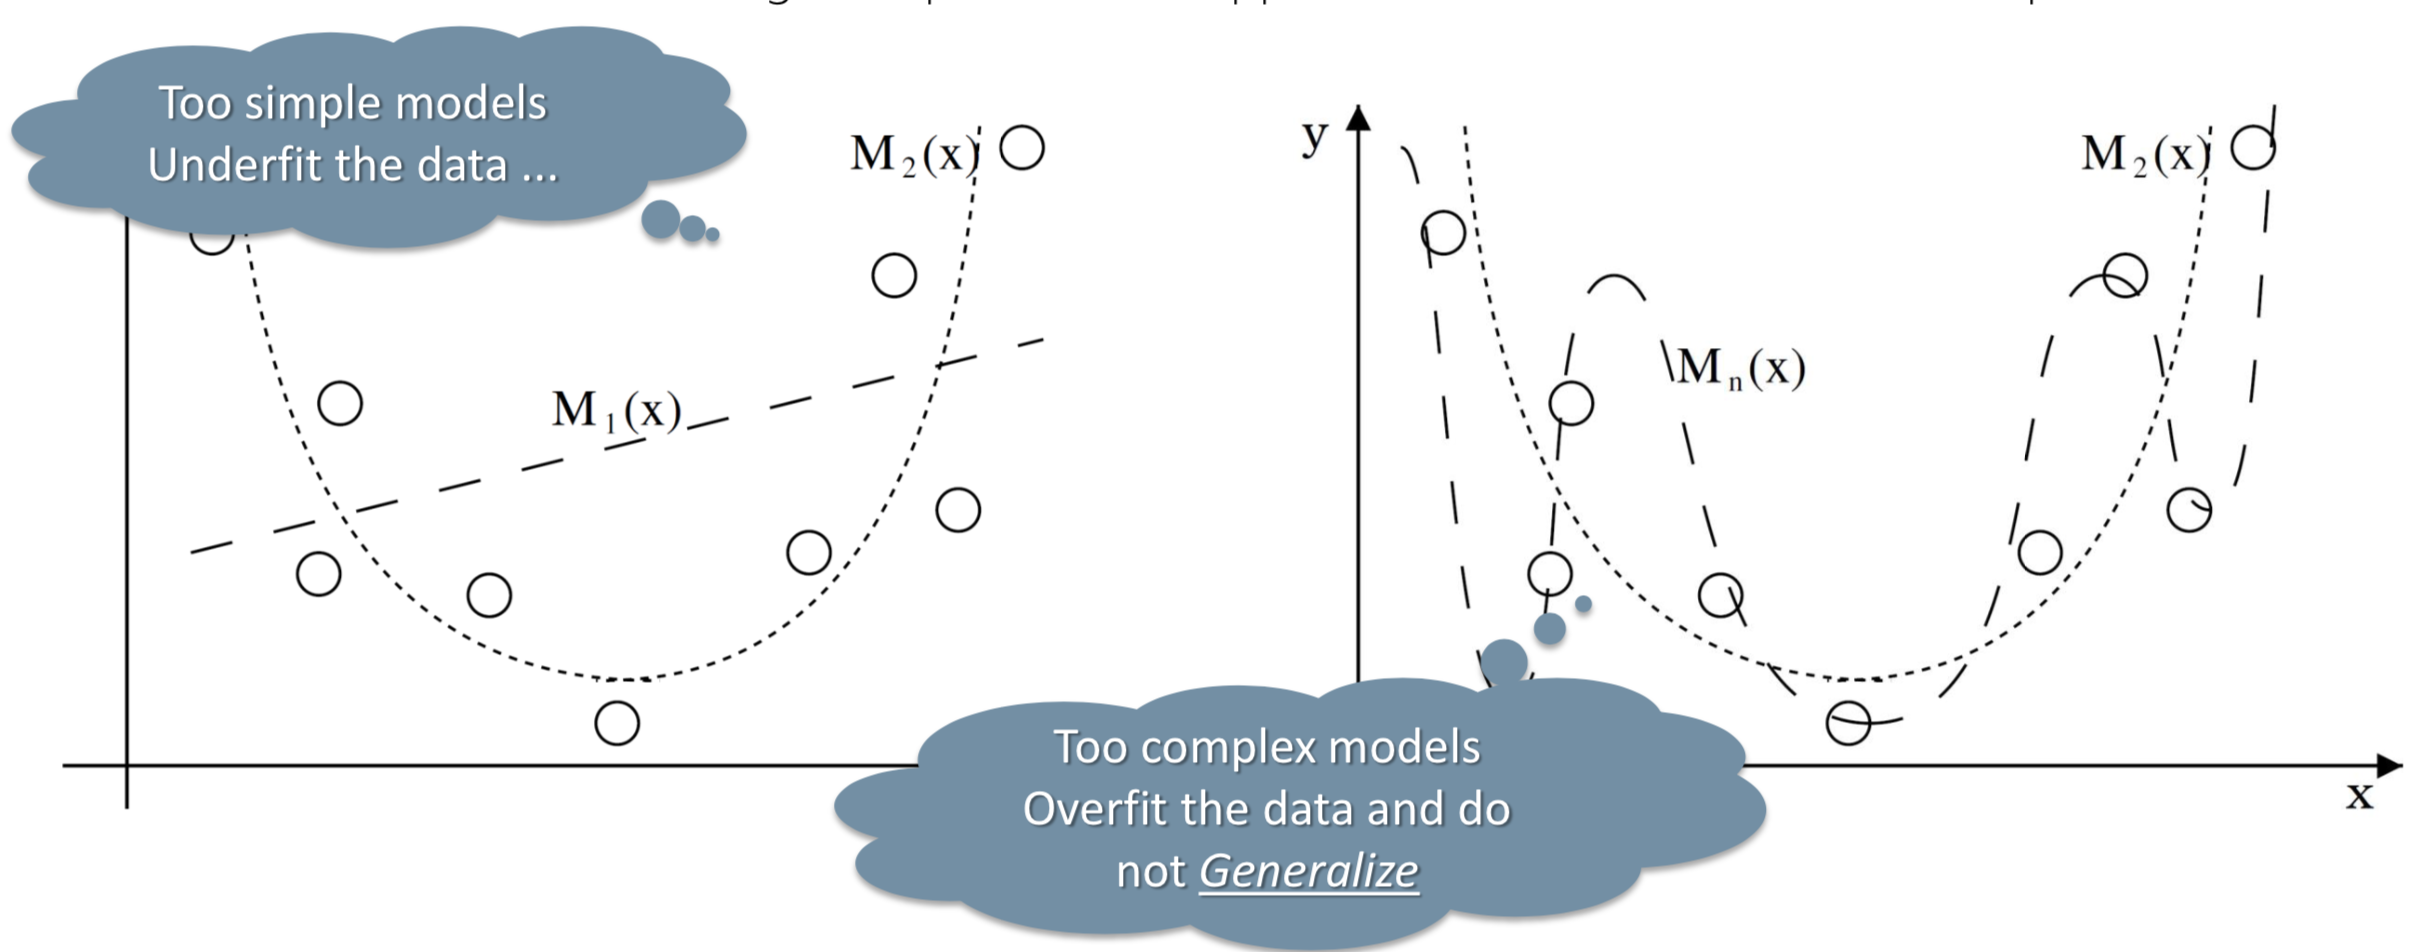
\includegraphics[width=15cm, height=6cm]{images/model_complexity.png}
    \caption{Under-fitting \& Over-fitting}
    \label{fig:model_complexity}
\end{figure}

 In fact, you tried to minimize the error on the train, but you lost the ability to generalize over new data: the model is not able to Generalize. It is an old story called Ockham's Razor: \textit{between a simple model and a very complex one you have to chose always the simple one}.\\
 In the other hand we have \textbf{Underfitting} when the model is too simple w.r.t. the real model. Too complex model tends to overfitting, so very good performance in training but very low performance in testing. You need to prevent overfitting.\\
 We need to find a way to measure the \textbf{Generalization}: training error/loss is not a good indicator of performance on future data:
 \begin{itemize}
     \item[--] The model has been learned from the very same training data, any estimate based on that data will be optimistic
     \item[--] New data will probably not be exactly the same as training data
    \item[--] You can find patterns even in random data
 \end{itemize}{}
 
 The idea is that you cannot use the same data of the training; you require a new independent set of data. Usually you take the data and split them in two sets: we train on one set and we test on the other. We \textit{never ever} use the test set at training time. Sometimes you can \textit{sample} the data \textit{with replacing}: it means that there is some probability for the same data to be in test and in train. This random sampling with replacing is called \textbf{Bootstrap} and it is used when the dataset is very small. What is important is that you want the training data to have the same distribution of your test data; what is done is \textbf{Stratified Sampling}: by doing it, essentially you are doing Cross Validation. The latter can have different form: hold-out set (but you have to be lucky to get a set that reflect the test set. With a small dataset, it could be problematic because the performance on test-set will depend on the separation taken into account), leave-one-out (not feasible for a huge amount of data), k-fold cross validation (averaging the performance of each fold).
 
 \subsection{Dealing with Overfitting}
Some of the strategies to deal with overfitting in neural network are presented in the following section:

\subsubsection{Early Stopping: Limiting Overfitting by Cross-Validation}
This is the most effective one if you have enough data. 
The point is that if you monitor the error on unseen data (validation-set) during the training process, you will reach a point in which your model has the minimum error on those new data. Once found this point, you can stop the training and consider it as the best model. To do this you need another set of data besides train and test: splitting the train-set, you get another train-set and a validation-set. The test set is used as the last thing to estimate the model on new data. The validation set is used during the training. You never use the validation to learn but only to stop the learning procedure.\\
To recap, \textit{Overfitting} networks show a \textbf{monotone} [decreasing] training error trend (on average
with SGD) as the number of gradient descent iterations \textbf{k}, but they lose generalization at some point, so we need to:
\begin{itemize}
    \item Hold out some data
    \item Train on the training set
    \item Perform cross-validation on the hold out set
    \item Stop train when validation error increases
\end{itemize}{}

One tipical procedure that is used to set up the neurons is to evaluate early stopping (the generalization error) to decide on other parameters, since the validation set error is an estimate of the error that you will get on test set. This idea of deciding on the parameters of the network is called \textbf{Hyper-parameter tuning}. Hyper-parameter describe the network structure and, once defined it, you know how many parameter you have to optimize. 

\subsubsection{Weights Regularization}
Sometimes you don't want to remove some data because you would like to exploit all of them. So there are technique to prevent overfitting without stopping the model, but instead somehow limiting the capability of the complex model: we have a powerful model but we impose some constraint on the model \textit{freedom}, based on a-priori assumption. \\
In case of neural network, we need to introduce a concept based on Bayesian Statistics: so far we have seen the problem of learning a model as a maximum learning estimation problem. We have been estimated the parameters of model in order to maximize the \textit{likelihood} of the data. What we show now is the difference between \textit{Frequentist} approach and \textit{Bayesian} approach. If we take the coin toss, the Frequentist approach bases the probabilities on the number of times I hit head/cross over the total number of tosses. The Bayesian approach has an opinion on the probabilities of head based on a bias (initially bias means that we assume that the coin is balanced, so we have 50\% head/cross); I toss the coin and I see head: the frequentist said that the prob. of head is $1$. The bayesian instead said $0.5$, one toss it is not enough to change the opinion. Second toss, second head: frequentiest said prob. of head is 1; bayesian said is not enough. After 10000 toss and 10000 heads the bayesian changes opinion. \\

According to the \underline{frequentist} approach, you have \underline{no opinion}: you look to the data and you select among all possible model the one that fits better the data $\rightarrow$ Unfortunately, this is basic overfitting, because you cannot bias the model. \\

On the other hand, the \underline{bayesian} approach starts from \underline{an opinion} that have a great \underline{bias}, and this prevent bayesianist to change opinion because he have seen only few data. \\

In statistics, opinions are named \textit{priors}. Maximum likelihood estimation finds the weights which maximize the data probability. A bayesianist looks for the most probable weights: in this way we are looking for \textbf{maximum a-posteriori}, we look for the most probable weights having observed data. The main difference between this two is that one looks for the probability of the data given the weights and the other for probability of the weights given the data. Substantially it is the \textbf{Bayes theorem}: $$
\begin{aligned}
w_{M A P} &=\operatorname{argmax}_{w} P(w | D) \\
&=\operatorname{argmax}_{w} P(D | w) \cdot P(w)
\end{aligned}
$$
This formula give you the possibility to bias the weights: i.e. if for you any weight is the same, this probability is uniform and you get maximum likelihood estimation because there is no difference between one and the other; if you want a model which is smooth, you have to put a prior probability which act as smoothy factor. \\
The idea of maximum a-posteriori is to force the model to select some weights and not other. It's sort of forcing, not a constraint. \\

How we define the prior in a way that our network does not overfit? It is observed in practice that \textit{small weights} makes network less prone to overfit; the bigger the weights the more likely the network overfit. Basically what we would like to do is limiting the capability of changing w.r.t. the variation on the input. \\
But what is that a small variation in the input become big in the output? The weights: they are the parameters, so they control the magnitude of the model.  That's why in general networks with small weights overfit less. We need to force our algorithm to prefer small weights: to do it, one possible way is to say that if you take all the weights, on average they have to be as small as possible, so near to zero on average. Then the bigger they become, the less likely they become. \\

One possible way to enforce bias on the weight distribution is to ask for the weight distribution as a Gaussian with zero-mean and some variance $\sigma_w^2$. \\
Instead of maximize likelihood we want to maximize a-posteriori probability, so we maximize the probability of the weights given the data. Let's assume we are in regression setting and the probabilities of weights are:
$$
P(w) \sim N\left(0, \sigma_{w}^{2}\right)
$$
$$
P(w) =  \frac{1}{\sqrt{2 \pi} \sigma_{w}} e^{-\frac{\left(w_{q}\right)^{2}}{2 \sigma_{w}^{2}}}
$$

Assume that $Q$ is the number of weights on the network (includes all the parameters in the network): 

$$
\begin{aligned}
\widehat{w} &=\operatorname{argmax}_{w} P(w | D)=\operatorname{argmax}_{w} P(D | w) P(w) \\
&=\operatorname{argmax}_{w} \prod_{n=1}^{N} \frac{1}{\sqrt{2 \pi} \sigma} e^{-\frac{\left(t_{n}-g\left(x_{n} | w\right)\right)^{2}}{2 \sigma^{2}}} \prod_{q=1}^{Q} \frac{1}{\sqrt{2 \pi} \sigma_{w}} e^{-\frac{\left(w_{q}\right)^{2}}{2 \sigma_{w}^{2}}} \\
&=\operatorname{argmin}_{w} \sum_{n=1}^{N} \frac{\left(t_{n}-g\left(x_{n} | w\right)\right)^{2}}{2 \sigma^{2}}+\sum_{q=1}^{Q} \frac{\left(w_{q}\right)^{2}}{2 \sigma_{w}^{2}} \\
&=\operatorname{argmin}_{w} \sum_{n=1}^{N}\left(t_{n}-g\left(x_{n} | w\right)\right)^{2}+\gamma \sum_{q=1}^{Q}\left(w_{q}\right)^{2}
\end{aligned}
$$

Where we define $\gamma = {\sigma^2 \over \sigma_w^2}$

The regularization term is positive. Adding a regularization term you are less prone to overfit because it makes your model smooth. \\
To force the network to have small weights we have to minimize the fit of the data plus some regularization term that is the sum of the squared of the weights $\rightarrow$ Ridge regression in Regression model does exactly this.\\ 
This is a classical form of loss function, another one is to add the sum of the absolute values of the weights $\rightarrow$ Lasso: it brings some weight to zero. \\

The best $\gamma$ is the one that minimize the generalization error: we can use Cross-Validation to select the proper $\gamma$. \\
In neural network literature, this approach that uses quadratic regularization term in error function is called \textbf{Weight Decay}. 





\subsubsection{Dropout}
By turning off randomly some neurons we force to learn an independent feature preventing hidden units to rely on other units (co-adaptation): each hidden unit is set to zero with $\boldsymbol{p_j^{(l)}}$ probability, e.g. $\boldsymbol{p_j^{(l)}} = 0.3$. \\
\textbf{Dropout} trains weaker classifiers, on different mini-batches and then at test time we implicitly average the responses of all ensemble members. At testing time we remove masks and average output (by weight scaling). \\
This technique modifies the network itself, not its loss function. It removes a small percentage of neurons on each hidden layer, chosen randomly.\\
It behaves as an ensemble method: it's like we have an ensemble of a lot of different networks. \\

\begin{minipage}{\linewidth}
        \centering
        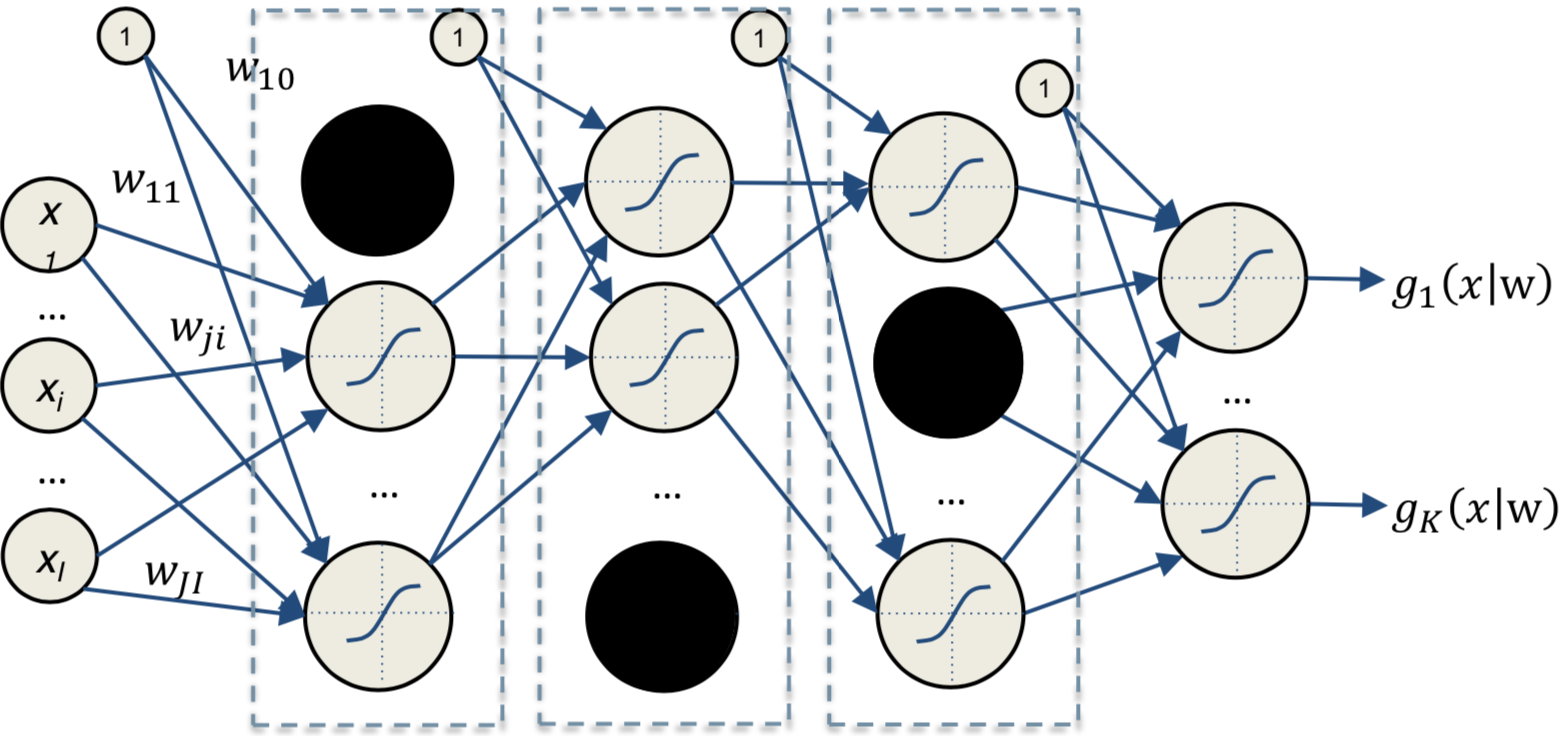
\includegraphics[width=13cm, height=5cm]{images/dropout.png}
        %\captionof{figure}{Logical Architecture}
        \label{fig:log_arch}
\end{minipage}\\



\subsection{Tips and Tricks}
Activation functions such as Sigmoid or Tanh saturate, which leads to:
\begin{itemize}
    \item[--] Gradient is close to zero
    \item[--] Backpropagation requires gradient multiplication
    \item[--] Gradient faraway from the output vanishes
    \item[--] Learning in deep networks does not happen
\end{itemize}{}

The problem of \textbf{Vanishing Gradient} raises from the fact that when you have very complex long neural network, to compute the gradient, you have to compute all the chain of derivatives:
$$
\frac{\left.\partial E\left(w_{j i}^{(1)}\right)\right)}{\partial w_{j i}^{(1)}}=-2 \sum_{n}^{N}\left(t_{n}-g_{1}\left(x_{n}, w\right)\right) \cdot g_{1}^{\prime}\left(x_{n}, w\right) \cdot w_{1 j}^{(2)} \cdot h_{j}^{\prime}\left(\sum_{j=0}^{J} w_{j i}^{(1)} \cdot x_{i, n}\right) \cdot x_{i}
$$
In deep networks, the gradient results in a very small number. \\
The issue is in Sigmoidal and Hyperbolic Tangent functions since the maximum of the derivative is in the origin and if we define they as a function $g()$, we know that 
\begin{itemize}
    \item for Sigmoid: $g'(a) = g(a)(1-g(a))$ $\rightarrow$ the maximum of the derivative is where the values is 0.5, so the maximum is equal to $0.5 (1 - 0.5) = 0.25$
    \item for Tanh: $g'(a) = 1 - g(a)^2$
\end{itemize}{}

In general the derivative is less than 1. The main issue with gradient descent is that the only way to fix it is by changing the operator function, so we need to use activation functions that do not suffer of this issue of having the derivative less than 1 $\Rightarrow$ \textbf{ReLU}

\subsubsection{ReLU}
\begin{wrapfigure}{r}{4cm}
    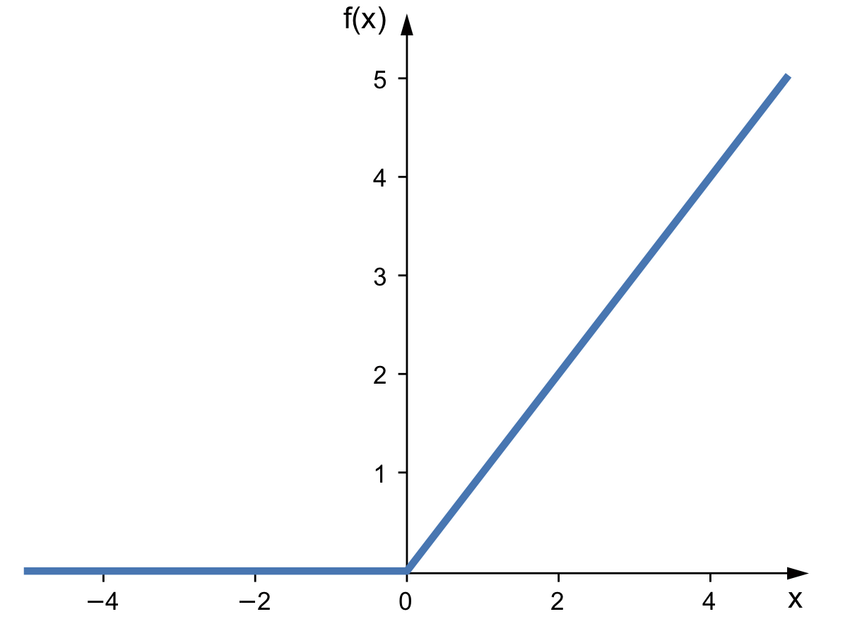
\includegraphics[width=5cm]{images/relu.png}
    %\label{fig:lstm_org}
\end{wrapfigure}  

The ReLU (Rectified Linear Unit) activation function is defined as:

$$ 
g(a) = ReLu(a) = max(0,a) 
$$ 

$$
g^{\prime (a)} = 1_{a>0}
$$ \\ \\

and it has some interesting properties:
\begin{itemize}
    \item[--] The derivative is either 1 or 0. Compute the derivative is essentially an "if"
    \item[--] Faster SGD Convergence: in the backward chaining, once you get the zero, you can forget about the past
    \item[--] Sparse activation (only part of hidden units are activated):  if on average half of the activation functions will be positive and the other half negative, then half of these neuron are switched off, so we don't have to compute it. Increase the efficiency and increase generalization since function is more simple, so it is more likely to not overfit.
    \item[--] Efficient gradient propagation (no vanishing or exploding gradient problems): you multiply by 1 or 0. 
    \item[--] Efficient computation (just thresholding at zero)
    \item[--] Scale-invariant: $max(0,a = a max(0,x)$. To some extent it is more robust to conditions, it is not affected by the values of current activation functions. 
    \item[--] It is not a linear function. 
\end{itemize}{}

But also potential disadvantages:
\begin{itemize}
    \item[--] Non-differentiable at zero: however it is differentiable (so not a significant issue)
    \item[--] Non-zero centered output: if you want the model outputs a number that is not strictly positive, you can use it. If you want a strictly positive output, you have to use a linear activation function.
    \item[--] Unbounded: Could potentially blow up
    \item[--] \textit{Dying Neurons}: ReLU neurons can sometimes be pushed into states in which they become inactive for essentially all inputs. No gradients flow backward through the neuron, and so the neuron becomes stuck and "dies", no way of switching it on. It decrease the model capacity and usually happens with high learning rates
\end{itemize}{}

Dying Neurons is an issue, but in the other hand switching off some neuron it's good since we create a simpler model. The problem is when it happens too early, i.e. at initialization time. Another thing that could happen: sometimes having a big learning rate could generate issues with these neurons because they become inactive too early w.r.t. training time.

%the derivative of g ... (guardare appunti dopo dropout). 
%Multiplying these number results in a very small number. The issue is in sigmoidal function or hyperbolic tangent since the maximum of the derivative is in the origin and if we define it as $g$, we know that for the sigmoid $g'(a) = g(a)(1-g(a))$, the maximum of the derivative is where the values is 0.5, so the maximum is equal to $0.5 (1 - 0.5) = 0.25$ [This is the maximum value]. In case of tanh the derivative is $g'(a) = 1 - g(a)^2$. So in general the derivative is less than 1. The main issue with gradient descent is that the only way to fix it is by changing the operator function. So we need to use activation functions that do not suffer of this issue of having the derivative less than 1 --> RELU: it has interisting properties: 
%\begin{itemize}
    %\item The derivative is 1: so the gradient are all either 1 o 0. So compute the derivative is an 'if'
    %\item Is not a linear function. 
    %\item In the backward chaining, once you get the zero, you can forget about the past (?) --> it is faster to compute with relu
    %\item You end up on sparse activation: if on average half of the activation function will be positive and the other half negative, on average half of these neuron are switched off, so we don't have to compute it. Increase the efficiency and increase generalization since function is more simple, so it is more likely to not overfit.
    %\item Efficient gradient propagation since there is no vanishing gradient and no exploding (it means when the derivative is greater than 1): in fact if you multiply number greater than 1, this number grows and grows and explodes resulting on unstable results. 
    %\item It is scale gradient, to some extent it is more robust to conditions, it is not affected by the values of current activation functions. 
%\end{itemize}{}

%Disadvantages:
%\begin{itemize}
%    \item It is not differentiable on zero: this is not significant issue
%    \item Non-zero centered output: if you want the model outputs a number that is not strictly positive, you can use it. If you want a strictly positive output, you have to use a linear activation function
%    \item It is unbounded: because of numerical optimization, it could grows unbounded
%    \item Dying neurons: the true issue. If you have the gradient equal to zero means that it will never change the weight. So if for some reason the gradient of this weight becomes zero, there will be no way of changing its weights, so there is no way to switch on this neuron. It is an issue, but in the other hand switching off some neuron it's good since we create a simpler model. The problem is when it happens too early, i.e. at inizialization time. Another thing that could happen: sometimes having a big learning rate could generate issues with these neurons because they become inactive too early wrt training time
%\end{itemize}{}

The main solutions are: 
\begin{itemize}
    \item Leaky RELU: the negative part decreases slowly, so there is a small gradient and when you go near or less than 0, you have a little chance to come back/to recover instead of switching itself off. It fix the "dying ReLU" \\
    \vspace{0.2cm}
    \begin{minipage}{\linewidth}
        \centering
        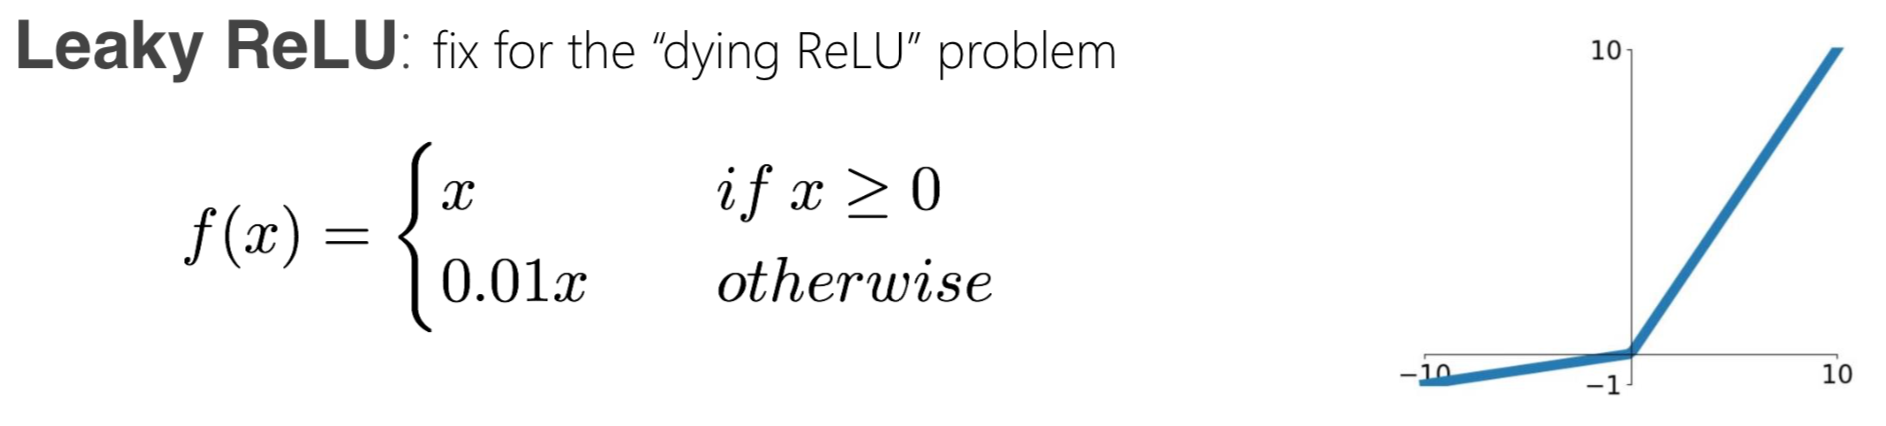
\includegraphics[width=14cm, height=3.5cm]{images/leaky_relu.png}
        %\captionof{figure}{The model pipeline.}
        %\label{fig:flow_fig}
    \end{minipage}

    \item ELU: you have an exponential and a lineal part and you can tune the $\alpha$ for the exponential part to define how much you would like to go under zero. It tries to make the mean activations closer to zero which speeds up learning. $\alpha$ hand by hand \\
    \vspace{0.2cm}
    \begin{minipage}{\linewidth}
        \centering
        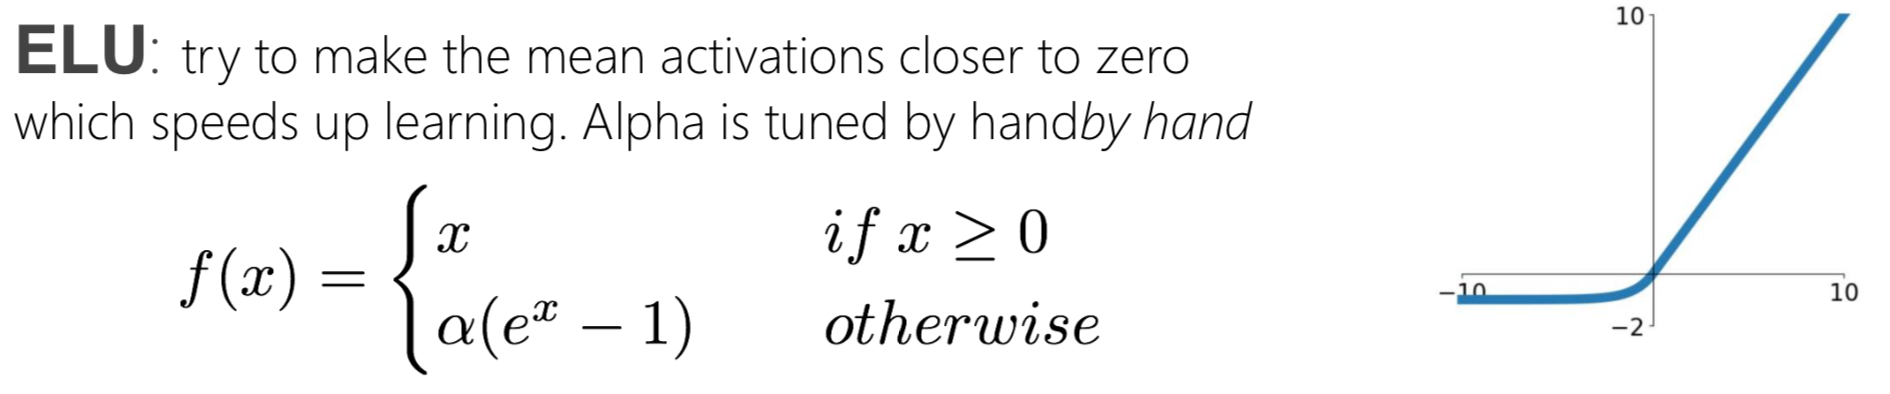
\includegraphics[width=14cm, height=3.5cm]{images/elu.png}
        %\captionof{figure}{The model pipeline.}
        %\label{fig:flow_fig}
    \end{minipage}
    
\end{itemize}{}

Modern architectures use ReLU, since initialization is a problem per-se.

\subsubsection{Weights Inizialization}
The final result of gradient descent is affected by weight initialization:
\begin{itemize}
    \item \textit{Zero}: it does not work. All gradient would be zero, no learning will happen. 
    \item \textit{Big Numbers}: bad idea. Assume to use sigmoid function and very big weights , you are in an area which gradient is close to zero $\rightarrow$ Long-time to converge
    \item \textit{Classic strategy}: small weights sampled by Gaussian distribution with zero mean and low variance. It works decently. The bigger is the variance the more it takes to training, since the weights are big and they are big when there are on the wrong side, so they take more time. Small number are fine: the weights starts more or less with the maximum of the gradient $\rightarrow$ at the very beginning the learning is fast. It is good for small networks, but it might be a problem for deeper neural networks.
\end{itemize}{}

However, in deep networks:
\begin{itemize}
    \item In a big network, if the weights are too small, you get the shrink gradient, since the gradient is the product of derivatives but also of the weights along a path. The gradient will not be zero but will be very small
    \item If you start with large weights, the gradient grows as it passes through the layers and at certain point will be too big. Assume you have a fixed learning rate, since in a way you tune the weights as (weight - learning rate * gradient), if the gradient grows, the product grows, so you have huge change in the weights. 
\end{itemize}{}

Some proposal to solve the problem is \textbf{Xavier Initialization}: \\
Suppose we have an input $x$ with $I$ components and a linear neuron with random weights $w$. The output of this neuron is
$$
h_{j}=w_{j 1} x_{1}+\cdots+w_{j i} x_{I}+\cdots+w_{j I} x_{I}
$$
We can derive that $w_{ji}x_{i}$ is going to have variance:
$$
\operatorname{Var}\left(w_{j i} x_{i}\right)=E\left[x_{i}\right]^{2} \operatorname{Var}\left(w_{j i}\right)+E\left[w_{j i}\right]^{2} \operatorname{Var}\left(x_{i}\right)+\operatorname{Var}\left(w_{j i}\right) \operatorname{Var}\left(x_{i}\right)
$$
%equal since it is a linear neuron, it is the weighted sum of the input. If you compute the variance of each of this element, what happen is that you are computing the variance of the weights and the input: the variance of weights * input is (formula slides).
Let's assume that both input and weights have zero-mean: 
$$
\operatorname{Var}\left(w_{j i} x_{i}\right)=\operatorname{Var}\left(w_{j i}\right) \operatorname{Var}\left(x_{i}\right)
$$
For the weights it is reasonable; for the input, it is not mandatory, but it has been observe that if you condition the input to have zero-mean and unitary variance, the optimization algorithm is better conditioned and it is more stable. 
%So it turns out that it is a product of variances (formula). 
If we assume all $w_i$ and $x_i$ are \textit{i.i.d} we obtain:
$$
\operatorname{Var}\left(h_{j}\right)=\operatorname{Var}\left(w_{j 1} x_{1}+\cdots+w_{j i} x_{I}+\cdots+w_{j I} x_{I}\right)=n \operatorname{Var}\left(w_{i}\right) \operatorname{Var}\left(x_{i}\right)
$$
So each neuron amplifies the variance of the input by a factor $nVar(w_i)$.\\
Assume that we have unitary variance input, what we don't want to do is to increase the variance of the input too much, so we try to force it to be consistently zero-mean and unitary along all the layers, we should enforce that the gain of the weights on each neuron should be 1: 
$$nVar(w_j) = 1$$
For this reason Xavier proposes to initialize 
$$w \sim N \left( 0,\frac{1}{n_{in}} \right)$$
More fast in converging and more stable.
%Make the assumption that all weigth are iid and all inputs are iid (formule). So each neuron amplifies n*Var(w) the variance of the input. Assume that we have unitary variance input, what we don't want to do is to increase the variance of the input too much, so we try to force to be consistently zero mean and unitary variance along all the layers: to do this we should enforce that the gain of the weights of each neuron should be 1, on average. 
%Spiegazione: assume I have the input and you can see the network as projecting the input in an higher dimensional space where I learn my model. If I make this zero-mean and unitary variance what happens is that at the very beginning I get n*Var(w), and so learning in this space may have conditioning properties, because in that space, weights and numbers are too big. So the fact that you normalize your input, it means that after one layer it explodes, because of this amplified effect on each neuron. To reduce the amplified effect, you want that the variance of the weights for that neuron multiplied by the number of input should be 1: by doing this, on average, what you get after the first layer has still zero-mean and unitary variance and after another layer has still zero-mean and unitary variance. The Xavier initialization propose to initialize the weights of each neuron sampling from a normal distribution with zero mean and a variance equal to 1/number of input [n] --> more fast in converge and more stable during training. 

Glorot and Bengio found a similar result: $n_{out}Var(w_j) = 1$, so they propose: 
$$w \sim N \left( 0,\frac{2}{n_{in} + n_{out}} \right)$$
More recently, He proposed, for rectified linear units:
$$w \sim N \left( 0,\frac{2}{n_{in}} \right)$$

\subsubsection{Momentum}
The idea is to accelerate training and giving to it some inertia.\\

\begin{wrapfigure}{r}{6cm}
    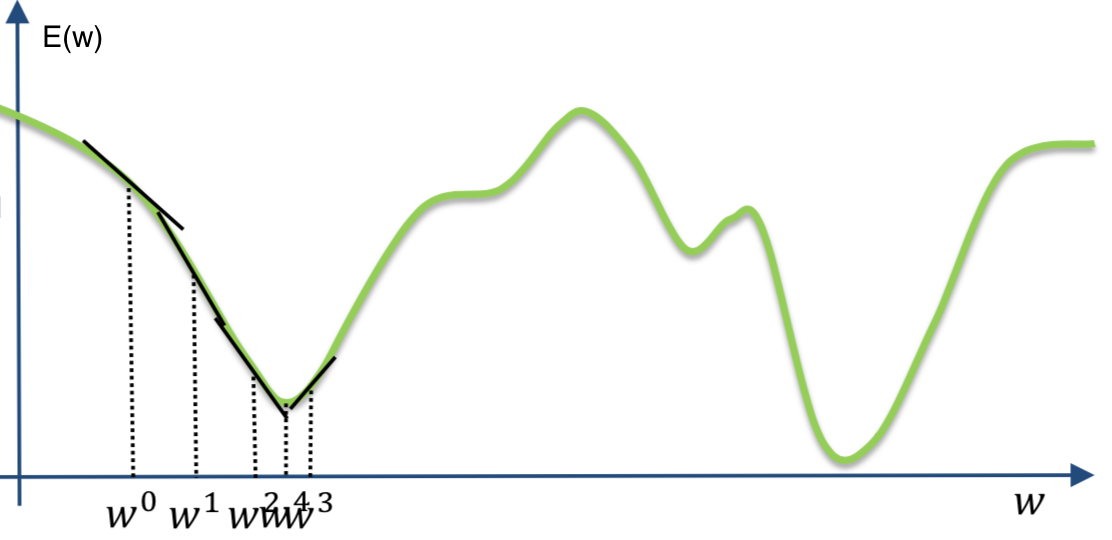
\includegraphics[width=6cm]{images/local_minima.png}
    %\label{fig:lstm_org}
\end{wrapfigure}  

Recalling Backpropagation, finding weights of a Neural Network is a non-linear minimization process: 
$$
\operatorname{argmin}_{w} E(w)=\sum_{n=1}^{N}\left(t_{n}-g\left(x_{n}, w\right)\right)^{2}
$$
We iterate from an initial configuration:
$$
w^{k+1}=w^{k}-\left.\eta \frac{\partial E(w)}{\partial w}\right|_{w^{k}}
$$

To avoid local minima we can use \textbf{Momentum}:
$$
w^{k+1}=w^{k}-\left.\eta \frac{\partial E(w)}{\partial w}\right|_{w^{k}}-\left.\alpha \frac{\partial E(w)}{\partial w}\right|_{w^{k-1}}
$$\\

\textbf{Nesterov Accelerated Gradient} makes a jump as momentum, then adjust
$$
w^{k+\frac{1}{2}}=w^{k}-\left.\alpha \frac{\partial E(w)}{\partial w}\right|_{w^{k-1}}
$$
$$
w^{k+1}=w^{k}-\left.\eta \frac{\partial E(w)}{\partial w}\right|_{w^{k+\frac{1}{2}}}
$$
The Nesterov idea is improving the estimate by dividing in two steps: the first step uses the momentum and it gives you a direction; in the second step re-estimate/update the gradient here, where the momentum leads you.\\
It should be a better estimate since the gradient will be closer to the minimum. It turns out to be more efficient, converges fast than SGD. \\

%There are 2 different algorithm, gradient descent and momentum. 
%\begin{itemize}
%    \item Nesterov Accelarated gradient: if you do standard momentum, you add to the gradient the momentum, so you have a sort of vector addiction which is the momentum. The point is that when you decide to compute the gradient, basically the idea is that you could improve on the estimate by dividing this two in two steps. The momentum gives you a direction where to move, so if you move that direction you will explore piece of error function which could give you more information about the gradient. Nesterov divides in two steps it, in the first half step you apply the momentum, so you move where the momentum lead you; the you re-estimate the gradient there, which should be a better estimate of the gradient closer to the minimum, and you update using the gradient there. It turns out to be more efficient, converge fast than SGD. So the idea is using the previous gradient to provide the better estimate where I should linearize my function. 
%\end{itemize}{}

There are other algorithms that try to \textbf{adapt learning rates} while learning, to deal with:
\begin{itemize}
    \item Gradient magnitudes vary across layers
    \item Early layers get "vanishing gradients": the gradient will be smaller and smaller the more you go back. It means that in the very first layer it should be boosted by an higher learning rate. 
    \item Should ideally use separate adaptive learning rates
\end{itemize}{}

Several algorithm are proposed: Rprop, Adagrad, RMSprop, AdaDelta and many others. \\
How they works? \\
Basically they study the error functions finding a lot of \textit{saddle points}: they are points in where you have two directional derivatives equal to 0, but in one direction it is a minimum, in the other is a maximum. Neural Networks have a lot of these points and having some stochasticity, which means not necessarily going directly to the minimum but having some noise, it will help a lot.

%there are other algorithm that tries to adapt learning rate while learning: the gradient is smaller and smaller the more you go on the back: it means that the information which arrives in the very first layer, should be boosted by the learning rate more at the one at very beginning. Also because the error close to the output, depends on all the error done before, so you should first fix the first weights and then the last one, otherwise you adapt on the error on the input before getting the solution. The idea is that each layer should have its own learning rate: but deciding the learning rate is very difficult in general, and decide it for each layer is impossible. So there are algorithm that adapt the learning rate. It means that the gradient keeps oscillating, it means that the learning rate is too big and you need to reduce it. Some of the algorithms, Adagrad, try to to adapt learning rate though time depending on the speed of convergence of the algorithm. Two most famous algorithm for this are Adagrad and Adam. How it works? (grafico appunti pag 31)
%This error function is called saddle since it contains saddle points: it is a point in where you have two directional derivatives = 0, but there is not the minimum: so in one direction is a minimum, in the other is a maximum. Neural Networks have a lot of these points: having some stochasticity, which means not necessarily going directly to the minimum but having some noise, it helps a lot. 

\subsubsection{Batch Normalization}
Networks converge faster if the inputs have been whitened (zero mean and unit variances) and are uncorrelated to account for \textit{covariate shift}. With Neural Networks we can have internal covariate shift so normalization could be useful also at the level of hidden layers.

Batch Normalization is a technique to cope with this:
\begin{itemize}
    \item[--] Leverages the fact that normalization is a differentiable
    \item[--] Forces activations throughout the network to take on a unit Gaussian at the beginning of the training
    \item[--] Adds a BatchNorm layer after fully connected layers (or convolutional layers), and before nonlinearities.
    \item Can be interpreted as doing preprocessing at every layer of the network, but integrated into the network itself in a differentiable way.
\end{itemize}{}

So the idea is to take the original data and normalize them centering the data with zero-mean and unitary variance for each feature. In that way you are sure that your data are in a square of size 1. This can be done for the input too. It is a specific layer network and you can have back-propagation even with this kind of layer  (which is removing the constant value and dividing by the constant value) because it is differentiable. You can learn or adapt the values of the mean and the variance. \\
In mini-batches, another relevant thing you would like to have is that all the batches have the same distribution, same mean and variance. The idea is to add as part of the training a normalization procedure: normalize the data as they pass through the layers. Obviously you can do it with Batch Normalization. \\

\vspace{0.2cm}
\begin{minipage}{\linewidth}
        \centering
        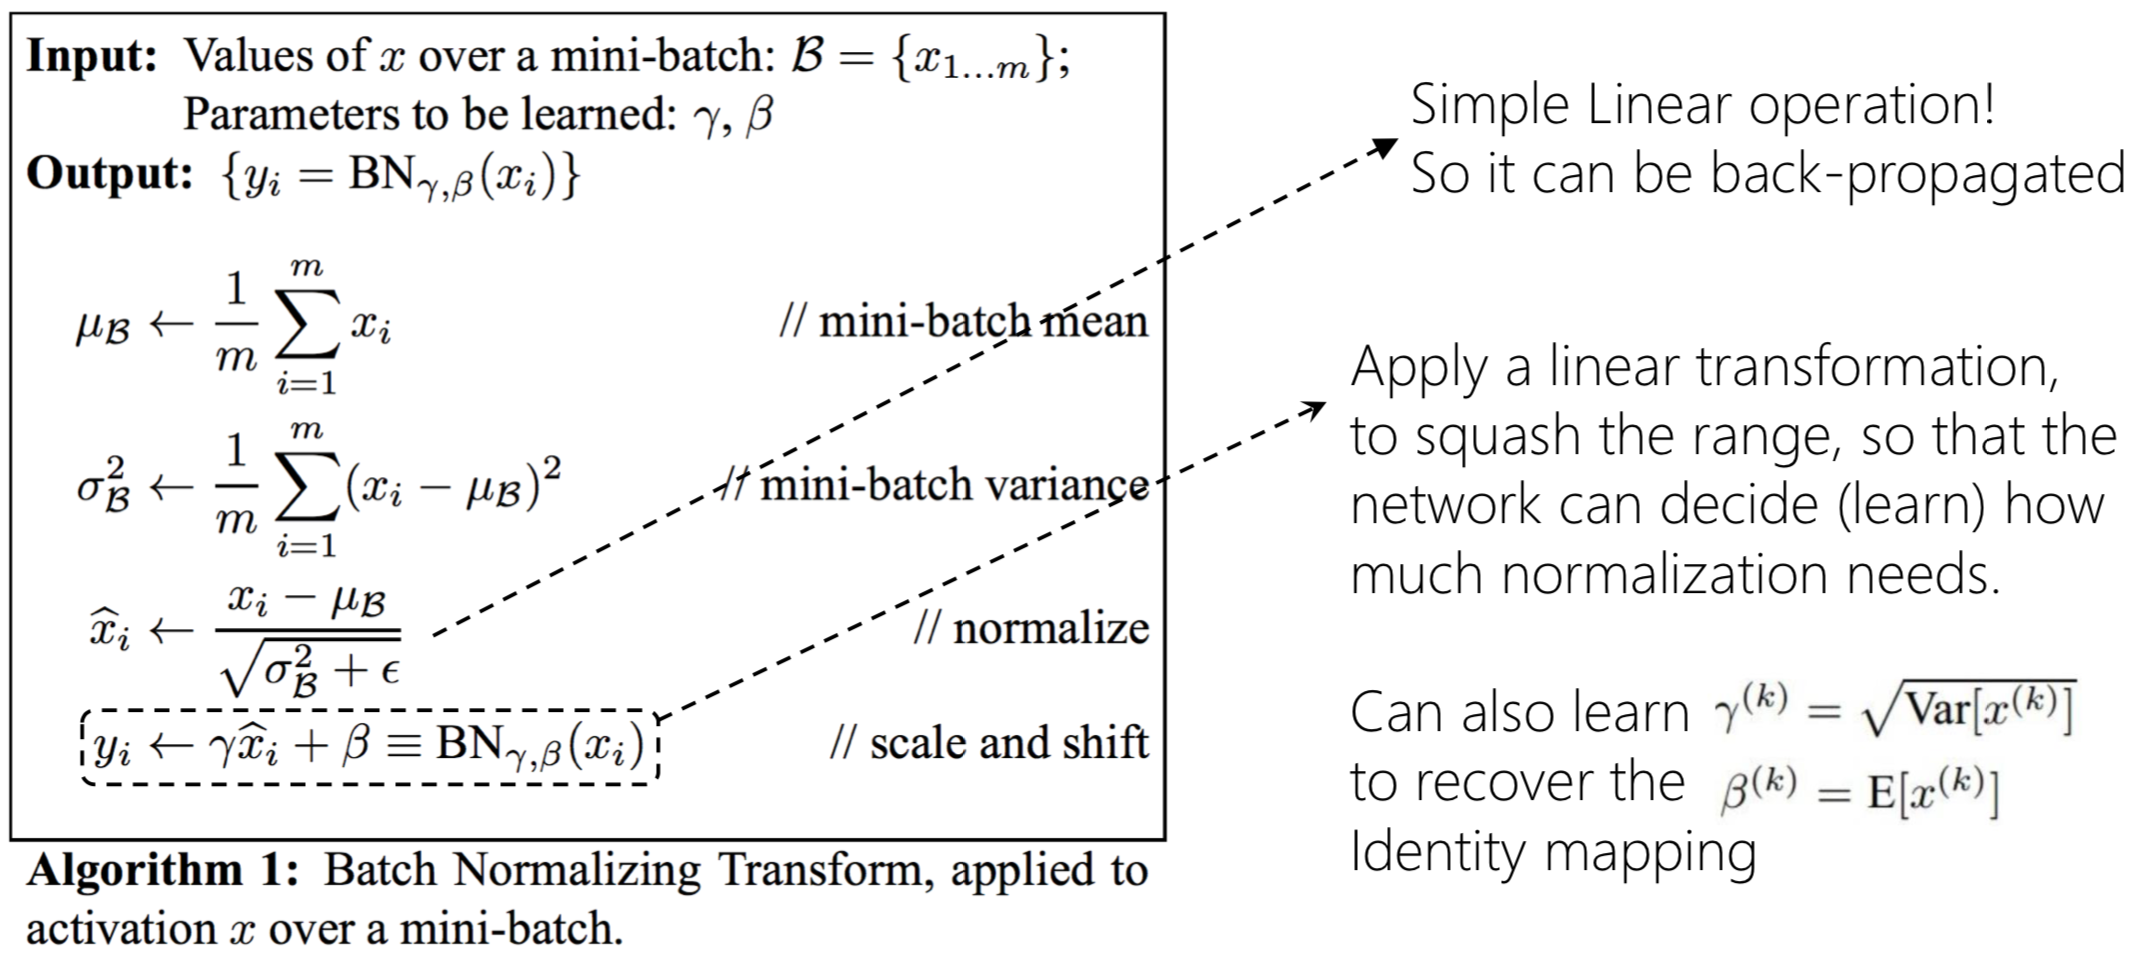
\includegraphics[width=14cm, height=6cm]{images/batch_norm.png}
        %\captionof{figure}{The model pipeline.}
        %\label{fig:flow_fig}
\end{minipage}
\vspace{0.2cm}


%It is a specific layer network. In practice, usually what you do is to normalize zero mean and unitary-variance of the input because it's known to be better in terms of 'covariance shift': if you have only shift in covariance, or in mean between the test and the training, if you normalize (they would be the same? reg.7 1:04:43). So the idea is that you take the original data and you normalize centering the data with zero mean and unitary variance for each of the feature, so you are sure that your data are in a square of size one. This is something that you can do for the input too. This may be useful in each level of representation.

%Another relevant thing is that want you would like to do with your data is to have the same distribution; in mini-batch training, you would like that all the batches have the same mean and the same variance. So the idea is to add as part of the training,  normalization procedure: you would like to normalize the data as they pass through the layer of the networks. This means that you want to force all the activation to take value as unitary-variance at the beginning of the training and during the training. To do this you can use what it is called Batch Normalization: it is something that can be put between the weighted sum of the input and non-linearity. Putting it in the middle, you have a normalization while you perform training. You can do back-propagation even if in the middle there is Batch Normalization layer since normalization (which is removing the constant value and dividing by the constant value) is differentiable. It is relevant because you can learn, or adapt, the number to substitute for the mean and the variance.

As you have noticed, during:
$
\widehat{x}_{i} \leftarrow \frac{x_{i}-\mu_{B}}{\sqrt{\sigma_{B}^{2}+\epsilon}}
$
we add some random noise to avoid division by zero.

In practice: 
\begin{enumerate}
    \item Each unit’s pre-activation is normalized (mean subtraction, stddev division)
    \item During training, mean and stddev is computed for each minibatch
    \item Backpropagation takes into account the normalization
    \item At test time, the global mean/stddev is used (global statistics are estimated using running averages during the training)
\end{enumerate}{}

It has shown to:
\begin{itemize}
    \item[--] Improve gradient flow through the network
    \item[--] Allows higher learning rates
    \item[--] Reduces the strong dependence on initialization
    \item[--] Acts as a form of regularization slightly reduces the need for dropout
\end{itemize}{}

%slide 33
%So what happens in batch normalization is more or less the following: each unit's pre-activation is normalized, it means you remove the mean and divide by the standard deviation. Then during the training you learn which is the mean and the standard deviation. At each mini-batch, you compute the mean and the standard deviation of the mini-batch. The mean is the mini-btach sum of the input, the mini-batch variance is (guardare pag 32). You update the data using these two numbers. You can also rescale and shift the output.  Qui

%$$
%\widehat{x}_{i} \leftarrow %\frac{x_{i}-\mu_{B}}{\sqrt{\sigma_{B}^{2}+\epsilon}}
%$$
%to avoid division by zero we add some random noise. So it is a huge differentiable mathematical formula, so you can derive the error wrt to this and you can learn the scale and the beta parameter used for this dataset and you should adapt through multiple mini-batch: at test time you have the global mean and the global standard deviation of the whole train. Basically this layer is normalizing the data within the batch having zero mean and unitary variance. 